\subsection{Manual 3 (15\%): Self-Signed SSL/TLS PKI and Browser Trust Remediation (Bonus)}
\label{subsec:manual3_pki}

Modern browsers enforce RFC~5280 X.509v3 certificate chain validation~\cite{rfc5280} and reject simple self-signed leaf certificates that lack Subject Alternative Name (SAN) extensions or a trusted Root Certificate Authority (CA) anchor. To satisfy the mandatory HTTPS encryption requirement over TLS~1.3~\cite{rfc8446} while earning the bonus credit for eliminating browser security warnings (\texttt{NET::ERR\_CERT\_AUTHORITY\_INVALID}), a two-tier private Public Key Infrastructure (PKI) was engineered using OpenSSL~\cite{openssl2024}, as depicted in Figure~\ref{fig:pki_architecture}.

\begin{figure*}[htbp]
\centering
\definecolor{pkiGoldFill}{HTML}{FEF3C7}
\definecolor{pkiGoldLine}{HTML}{B45309}
\definecolor{pkiGoldBg}{HTML}{FFFBEB}
\definecolor{pkiBlueFill}{HTML}{DBEAFE}
\definecolor{pkiBlueLine}{HTML}{1D4ED8}
\definecolor{pkiBlueBg}{HTML}{EFF6FF}
\definecolor{pkiIndigoFill}{HTML}{E0E7FF}
\definecolor{pkiIndigoLine}{HTML}{3730A3}
\definecolor{pkiPurpleFill}{HTML}{EDE9FE}
\definecolor{pkiPurpleLine}{HTML}{6D28D9}
\definecolor{pkiPurpleBg}{HTML}{F5F3FF}
\definecolor{pkiGreenFill}{HTML}{D1FAE5}
\definecolor{pkiGreenLine}{HTML}{047857}
\definecolor{pkiGreenBg}{HTML}{ECFDF5}
\definecolor{pkiRedFill}{HTML}{FEE2E2}
\definecolor{pkiRedLine}{HTML}{B91C1C}
\definecolor{pkiSlateFill}{HTML}{F1F5F9}
\definecolor{pkiSlateLine}{HTML}{475569}

\resizebox{0.96\textwidth}{!}{%
\begin{tikzpicture}[
    >=Stealth,
    every node/.style={font=\scriptsize, text=black!88},
    node distance=0.45cm and 0.55cm,
    card/.style={
        rectangle, rounded corners=3pt, draw=pkiSlateLine, fill=white,
        line width=0.75pt, inner sep=5.5pt, align=left
    },
    card_gold/.style={card, draw=pkiGoldLine, fill=white},
    card_blue/.style={card, draw=pkiBlueLine, fill=white},
    card_indigo/.style={card, draw=pkiIndigoLine, fill=pkiIndigoFill!35},
    card_purple/.style={card, draw=pkiPurpleLine, fill=white},
    card_green/.style={card, draw=pkiGreenLine, fill=white},
    card_err/.style={card, draw=pkiRedLine, fill=pkiRedFill!75, align=center},
    card_ok/.style={card, draw=pkiGreenLine, fill=pkiGreenFill!85, align=center},
    hdr_pill/.style={
        rectangle, rounded corners=2pt, font=\scriptsize\bfseries,
        inner xsep=6pt, inner ysep=2.5pt, text=white
    },
    zone_box/.style={
        rectangle, rounded corners=6pt, dashed, line width=0.85pt, inner sep=8pt
    },
    flow_arr/.style={
        -{Stealth[length=5pt, width=3.5pt]},
        line width=0.95pt, color=pkiSlateLine, shorten >=1.5pt, shorten <=1pt
    },
    flow_short/.style={
        -{Stealth[length=4pt, width=2.8pt]},
        line width=0.85pt, color=pkiSlateLine, shorten >=1pt, shorten <=0.5pt
    },
    rail_gold/.style={
        -{Stealth[length=5pt, width=3.5pt]},
        line width=0.95pt, color=pkiGoldLine, rounded corners=4pt, shorten >=1.5pt
    },
    verify_arr/.style={
        {Stealth[length=4.5pt, width=3pt]}-{Stealth[length=4.5pt, width=3pt]},
        line width=0.95pt, densely dashed, color=pkiGreenLine, shorten >=1.5pt, shorten <=1.5pt
    },
    edge_tag/.style={
        font=\tiny\bfseries, fill=white, inner xsep=3.5pt, inner ysep=1.5pt,
        rounded corners=1.5pt, draw=black!20, line width=0.35pt, align=center
    },
]

\node[card_gold, text width=6.6cm, minimum height=2.15cm] (ca_id) at (0,0) {%
    \textbf{\footnotesize COIL Group 2 Root CA}\\[2pt]
    {\tiny\color{pkiGoldLine}\textbf{Self-Signed Root Authority (Offline)}}\\[3pt]
    $\bullet$ \textbf{Subject/Issuer:} \texttt{CN = COIL Group 2 Root CA}\\
    $\bullet$ \textbf{Cert:} \texttt{COIL\_Group2\_Root\_CA.crt} / \texttt{ca-cert.pem}\\
    $\bullet$ \textbf{Signing Key:} \texttt{ca-key.pem} (offline private key)
};

\node[card_gold, text width=7.1cm, minimum height=2.15cm, right=0.55cm of ca_id] (ca_specs) {%
    \textbf{Cryptographic Profile \& X.509v3 Constraints}\\[3pt]
    $\bullet$ \textbf{Key / Hash:} \texttt{2048-bit RSA}, SHA-256 self-signed\\
    $\bullet$ \textbf{Extensions:} \texttt{CA:TRUE}, \texttt{keyCertSign}, \texttt{cRLSign}\\
    $\bullet$ \textbf{Serial:} \texttt{1CB6...57D0}\\
    $\bullet$ \textbf{Validity:} Nov 21, 2026 -- Nov 18, 2036 (\qty{3650}{days})
};

\coordinate (t1_mid_top) at ($(ca_id.north west)!0.5!(ca_specs.north east)$);
\coordinate (t1_mid_bot) at ($(ca_id.south west)!0.5!(ca_specs.south east)$);

\node[hdr_pill, fill=pkiGoldLine, anchor=south west] (t1_hdr)
    at ($(ca_id.north west)+(0,0.18cm)$)
    {TIER 1: Offline Root Authority};

\begin{pgfonlayer}{background}
    \node[zone_box, draw=pkiGoldLine, fill=pkiGoldBg, fit=(t1_hdr)(ca_id)(ca_specs)] (zone_t1) {};
\end{pgfonlayer}

\node[rectangle, rounded corners=3pt, fill=pkiSlateFill, draw=pkiSlateLine!45,
      line width=0.6pt, inner xsep=12pt, inner ysep=4pt,
      font=\small\bfseries, text=black!90, anchor=south] (fig_title)
    at ($(zone_t1.north -| t1_mid_top)+(0,0.42cm)$)
    {COIL Group 2 -- Custom Root CA PKI, X.509v3 SANs, TLS 1.3 Stack \& Trust Remediation};

\coordinate (t2_row_top) at ($(zone_t1.south -| t1_mid_bot)+(0,-1.65cm)$);

\node[card_blue, text width=4.45cm, minimum height=3.20cm, anchor=north] (leaf_crt)
    at (t2_row_top) {%
    \textbf{Leaf Certificate (\texttt{server.crt})}\\[2pt]
    \textbf{Subject:} \texttt{CN = www.coil-group2.com}\\[3pt]
    $\bullet$ \textbf{Constraints:} \texttt{CA:FALSE}\\
    $\bullet$ \textbf{Key Usage:} \texttt{digitalSignature},\\
    \hspace*{1.2em}\texttt{keyEncipherment}\\
    $\bullet$ \textbf{EKU:} \texttt{serverAuth}, \texttt{clientAuth}\\
    $\bullet$ \textbf{Serial:} \texttt{173D...87D7}\\
    $\bullet$ \textbf{Valid:} Nov 21, 2026 -- Feb 23, 2029\\
    \hspace*{1.2em}(\qty{825}{days})
};

\node[card_blue, text width=3.05cm, minimum height=1.42cm, anchor=north east] (t2_cnf)
    at ($(leaf_crt.north west)+(-0.65cm,0)$) {%
    \textbf{OpenSSL Policy}\\[2pt]
    \texttt{openssl.cnf}\\
    {\tiny Profiles: \texttt{[v3\_ca]} \& \texttt{[server\_ext]}}
};

\node[card_blue, text width=3.05cm, minimum height=1.42cm, anchor=south east] (t2_csr)
    at (leaf_crt.south west -| t2_cnf.east) {%
    \textbf{Signing Request}\\[2pt]
    \texttt{server.csr}\\
    {\tiny Signed by \texttt{ca-key.pem}}
};

\node[card_indigo, text width=4.05cm, minimum height=3.20cm, anchor=north west] (san_box)
    at ($(leaf_crt.north east)+(0.95cm,0)$) {%
    \textbf{X.509v3 SAN Extension}\\[1pt]
    {\tiny\color{pkiIndigoLine}\textbf{Subject Alternative Name (\texttt{[alt\_names]})}}\\[3pt]
    \textbf{DNS Entries (5):}\\
    {\tiny\texttt{www.coil-group2.com}\\[0.5pt]
    \texttt{coil-group2.com}\\[0.5pt]
    \texttt{unillanos.coil-group2.com}\\[0.5pt]
    \texttt{seneca.coil-group2.com}\\[0.5pt]
    \texttt{localhost}}\\[3pt]
    \textbf{IP Entries (4):}\\
    {\tiny\texttt{172.22.201.2}, \texttt{172.22.31.69},\\[0.5pt]
    \texttt{10.51.76.174}, \texttt{127.0.0.1}}
};

\node[hdr_pill, fill=pkiBlueLine, anchor=south west] (t2_hdr)
    at ($(t2_cnf.north west)+(0,0.18cm)$)
    {TIER 2: OpenSSL \& Leaf CA};

\begin{pgfonlayer}{background}
    \node[zone_box, draw=pkiBlueLine, fill=pkiBlueBg, fit=(t2_hdr)(t2_cnf)(t2_csr)(leaf_crt)(san_box)] (zone_t2) {};
\end{pgfonlayer}

\def\coloffset{4.90cm}
\coordinate (t3_top_y) at ($(zone_t2.south -| t1_mid_bot)+(0,-1.75cm)$);
\coordinate (t3A_center_top) at ($(t3_top_y)+(-\coloffset,0)$);
\coordinate (t3B_center_top) at ($(t3_top_y)+(+\coloffset,0)$);

\node[card_purple, text width=6.95cm, minimum height=1.05cm, anchor=north] (pA_bundle) at (t3A_center_top) {%
    \textbf{TLS Certificate Chain \& Private Key Bundle}\\[2pt]
    \texttt{fullchain.pem} (\texttt{server.crt} + \texttt{ca-cert.pem}) + \texttt{server-key.pem}
};

\node[card_purple, text width=6.95cm, minimum height=1.28cm, below=0.45cm of pA_bundle] (pA_ctx) {%
    \textbf{Python HTTPS Server Context}\\[2pt]
    \texttt{ssl.SSLContext(PROTOCOL\_TLS\_SERVER)}\\
    ALPN: \texttt{http/1.1} \quad$\cdot$\quad Cipher: \texttt{TLS\_AES\_256\_GCM\_SHA384}
};

\coordinate (row3_top_y) at ($(pA_ctx.south)+(0,-0.55cm)$);

\node[card_purple, text width=3.20cm, minimum height=1.18cm, align=center, anchor=north west] (pA_uni)
    at (pA_ctx.west |- row3_top_y) {%
    \textbf{UniLlanos Server}\\
    \texttt{172.22.201.2:443}
};

\node[card_purple, text width=3.20cm, minimum height=1.18cm, align=center, anchor=north east] (pA_sen)
    at (pA_ctx.east |- row3_top_y) {%
    \textbf{Seneca Gateway}\\
    \texttt{172.22.31.69:443}
};

\node[hdr_pill, fill=pkiPurpleLine, anchor=south west] (pA_hdr)
    at ($(pA_bundle.north west)+(0,0.18cm)$)
    {TIER 3A: Server TLS 1.3 Stack};

\begin{pgfonlayer}{background}
    \node[zone_box, draw=pkiPurpleLine, fill=pkiPurpleBg, fit=(pA_hdr)(pA_bundle)(pA_ctx)(pA_uni)(pA_sen)] (zone_3A) {};
\end{pgfonlayer}

\node[card_green, text width=6.95cm, minimum height=1.05cm, anchor=north] (pB_dist) at (t3B_center_top) {%
    \textbf{Root CA Distribution Mechanism}\\[2pt]
    \texttt{COIL\_Group2\_Root\_CA.crt} (served via \texttt{/ca.crt} or \texttt{install\_root\_ca.ps1})
};

\node[card_green, text width=3.85cm, minimum height=1.28cm, anchor=north west] (pB_win)
    at ($(pB_dist.south west)+(0,-0.45cm)$) {%
    \textbf{Windows Trust Store}\\
    \texttt{Cert:\textbackslash LocalMachine\textbackslash Root}\\
    {\tiny Thumbprint: \texttt{6C94...E0D9}}
};

\node[card_green, text width=2.55cm, minimum height=1.28cm, anchor=north east] (pB_and)
    at ($(pB_dist.south east)+(0,-0.45cm)$) {%
    \textbf{Android OS}\\
    Android Trusted\\
    Credentials
};

\node[card_err, text width=3.22cm, minimum height=1.18cm, anchor=north west] (pB_err)
    at (pB_dist.west |- row3_top_y) {%
    \textbf{Eliminates Warning}\\[2pt]
    {\fontsize{4.6}{6}\selectfont\texttt{NET::ERR\_CERT\_AUTHORITY\_INVALID}}
};

\node[card_ok, text width=2.45cm, minimum height=1.18cm, anchor=north east] (pB_ok)
    at (pB_dist.east |- row3_top_y) {%
    \textbf{Verified Trusted}\\
    \textbf{HTTPS Padlock}\\
    {\tiny Chrome \& Mobile}
};

\node[hdr_pill, fill=pkiGreenLine, anchor=south west] (pB_hdr)
    at ($(pB_dist.north west)+(0,0.18cm)$)
    {TIER 3B: Client Trust Store (Bonus)};

\begin{pgfonlayer}{background}
    \node[zone_box, draw=pkiGreenLine, fill=pkiGreenBg, fit=(pB_hdr)(pB_dist)(pB_win)(pB_and)(pB_err)(pB_ok)] (zone_3B) {};
\end{pgfonlayer}

\coordinate (t1_sign_exit) at (zone_t1.south -| leaf_crt.north);
\draw[flow_arr] (t1_sign_exit) -- (leaf_crt.north);
\node[edge_tag] at ($(t1_sign_exit)!0.50!(t1_sign_exit |- zone_t2.north)$)
    {Signs CSR w/ \texttt{ca-key.pem}};

\coordinate (t2_join) at ($(leaf_crt.west)+(-0.32cm,0)$);
\draw[line width=0.85pt, color=pkiSlateLine] (t2_cnf.east) -| (t2_join);
\draw[line width=0.85pt, color=pkiSlateLine] (t2_csr.east) -| (t2_join);
\draw[flow_short] (t2_join) -- (leaf_crt.west);

\draw[flow_short] (leaf_crt.east) -- node[edge_tag, above=4pt] {Embeds} (leaf_crt.east -| san_box.west);

\coordinate (pA_crt_in) at ($(pA_bundle.north east)+(-0.95cm,0)$);
\coordinate (bus_t2_t3) at ($(zone_t2.south)!0.50!(zone_3A.north)$);
\draw[flow_arr, rounded corners=4pt]
    (leaf_crt.south) -- (leaf_crt.south |- bus_t2_t3)
    -| (pA_crt_in);
\node[edge_tag] at ($(leaf_crt.south |- bus_t2_t3)!0.48!(pA_crt_in |- bus_t2_t3)$)
    {\texttt{server.crt} (Leaf)};

\coordinate (rail_L_x) at ($(zone_3A.west)+(-0.62cm,0)$);
\draw[rail_gold]
    (zone_t1.west) -- (zone_t1.west -| rail_L_x)
    |- (pA_bundle.west);
\node[edge_tag, text=pkiGoldLine, draw=pkiGoldLine!60, anchor=center]
    at (rail_L_x |- leaf_crt.center)
    {\texttt{ca-cert.pem}\\[1pt](Chain Anchor)};

\coordinate (rail_R_x) at ($(zone_3B.east)+(0.62cm,0)$);
\draw[rail_gold]
    (zone_t1.east) -- (zone_t1.east -| rail_R_x)
    |- (pB_dist.east);
\node[edge_tag, text=pkiGoldLine, draw=pkiGoldLine!60, anchor=center]
    at (rail_R_x |- san_box.center)
    {\texttt{COIL\_Group2\_}\\[1pt]\texttt{Root\_CA.crt}\\[1pt](Trust Anchor)};

\draw[flow_short] (pA_bundle.south) -- (pA_ctx.north);
\coordinate (pA_split) at ($(pA_ctx.south)!0.45!(pA_uni.north -| pA_ctx.south)$);
\draw[line width=0.85pt, color=pkiSlateLine] (pA_ctx.south) -- (pA_split);
\draw[flow_short, rounded corners=3pt] (pA_split) -| (pA_uni.north);
\draw[flow_short, rounded corners=3pt] (pA_split) -| (pA_sen.north);

\coordinate (pB_split) at ($(pB_dist.south)!0.45!(pB_win.north -| pB_dist.south)$);
\draw[line width=0.85pt, color=pkiSlateLine] (pB_dist.south) -- (pB_split);
\draw[flow_short, rounded corners=3pt] (pB_split) -| (pB_win.north);
\draw[flow_short, rounded corners=3pt] (pB_split) -| (pB_and.north);

\draw[flow_short] (pB_win.south) -- (pB_win.south |- pB_err.north);
\draw[flow_short] (pB_and.south) -- (pB_and.south |- pB_ok.north);
\draw[flow_short, color=pkiGreenLine] (pB_err.east) -- (pB_ok.west);

\draw[verify_arr] (pA_sen.east) -- (pB_err.west);
\node[edge_tag, text=pkiGreenLine, draw=pkiGreenLine!60, anchor=south]
    at ($(pA_sen.east)!0.5!(pB_err.west)+(0,0.14cm)$)
    {TLS 1.3 +\\[1pt]SAN Match};

\coordinate (bot_mid) at ($(zone_3A.south west)!0.5!(zone_3B.south east)+(0,-0.45cm)$);

\node[font=\scriptsize\bfseries, anchor=north] (leg_hdr) at (bot_mid)
    {Architecture Legend \& Cryptographic Flow Semantics};

\node[font=\tiny, anchor=north, align=center] (leg_r1) at ($(leg_hdr.south)+(0,-0.12cm)$) {%
    \fcolorbox{pkiGoldLine}{pkiGoldBg}{\rule{0pt}{4.2pt}\rule{6.5pt}{0pt}}\, Tier 1: Offline Root CA \qquad
    \fcolorbox{pkiBlueLine}{pkiBlueBg}{\rule{0pt}{4.2pt}\rule{6.5pt}{0pt}}\, Tier 2: OpenSSL Policy \& SAN Leaf \qquad
    \fcolorbox{pkiPurpleLine}{pkiPurpleBg}{\rule{0pt}{4.2pt}\rule{6.5pt}{0pt}}\, Tier 3A: Server TLS 1.3 Stack \qquad
    \fcolorbox{pkiGreenLine}{pkiGreenBg}{\rule{0pt}{4.2pt}\rule{6.5pt}{0pt}}\, Tier 3B: Client Trust Store (Bonus)
};

\coordinate (leg_r2_y) at ($(leg_r1.south)+(0,-0.32cm)$);

\node[font=\tiny, anchor=west] (ar2_txt) at ($(leg_r2_y)+(-0.95cm,0)$) {Root CA Distribution Rail};
\draw[rail_gold] ($(ar2_txt.west)+(-0.72cm,0)$) -- ($(ar2_txt.west)+(-0.06cm,0)$);
\coordinate (ar2_start) at ($(ar2_txt.west)+(-0.75cm,0)$);

\node[font=\tiny, anchor=east] (ar1_txt) at ($(ar2_start)+(-0.90cm,0)$) {Signing / Deployment Flow};
\draw[flow_short] ($(ar1_txt.west)+(-0.72cm,0)$) -- ($(ar1_txt.west)+(-0.06cm,0)$);
\coordinate (ar1_start) at ($(ar1_txt.west)+(-0.75cm,0)$);

\node[font=\tiny, anchor=west] (ar3_txt) at ($(ar2_txt.east)+(1.62cm,0)$) {Verified TLS 1.3 Chain \& SAN Handshake};
\draw[verify_arr] ($(ar3_txt.west)+(-0.72cm,0)$) -- ($(ar3_txt.west)+(-0.06cm,0)$);

\coordinate (leg_flush_L) at (zone_3A.west |- leg_hdr.north);
\coordinate (leg_flush_R) at (zone_3B.east |- ar3_txt.south);

\begin{pgfonlayer}{background}
    \node[rectangle, rounded corners=4pt, draw=pkiSlateLine!45, fill=pkiSlateFill,
          line width=0.6pt, inner xsep=0pt, inner ysep=5pt,
          fit=(leg_flush_L)(leg_flush_R)(leg_hdr)(leg_r1)(ar1_start)(ar3_txt)] (legend_bar) {};
\end{pgfonlayer}

\end{tikzpicture}%
}
\caption{Three-tier Public Key Infrastructure (PKI) and browser trust remediation architecture. Tier~1 establishes the offline 2048-bit RSA \texttt{COIL Group 2 Root CA} (\qty{3650}{days}); Tier~2 signs the leaf certificate (\texttt{server.crt}, \qty{825}{days}) with five DNS and four IPv4 Subject Alternative Names (SANs); Tier~3A deploys \texttt{fullchain.pem} to the dual-node TLS~1.3 server stack while Tier~3B imports \texttt{COIL\_Group2\_Root\_CA.crt} into Windows and Android root trust stores to eliminate \texttt{NET::ERR\_CERT\_AUTHORITY\_INVALID} warnings (bonus criterion).}
\label{fig:pki_architecture}
\end{figure*}


\subsubsection{Step 1: OpenSSL X.509v3 Configuration Policy (\texttt{openssl.cnf})}
Create the OpenSSL configuration file \texttt{modulo2/certificados/openssl.cnf} defining two distinct X.509v3 extension profiles: \texttt{[v3\_ca]} for the offline Root CA (\texttt{basicConstraints = critical, CA:true}, \texttt{keyUsage = critical, digitalSignature, cRLSign, keyCertSign}) and \texttt{[server\_ext]} for the multi-tenant server leaf certificate (\texttt{basicConstraints = CA:FALSE}, \texttt{extendedKeyUsage = serverAuth, clientAuth}, and \texttt{subjectAltName = @alt\_names}). The SAN block binds all five DNS hostnames and four IPv4 addresses used across the SD-WAN overlay:

\begin{lstlisting}[caption={X.509v3 Subject Alternative Name declaration in \texttt{openssl.cnf}.},label={lst:manual3_san}]
[ server_ext ]
subjectKeyIdentifier   = hash
authorityKeyIdentifier = keyid,issuer
basicConstraints       = CA:FALSE
keyUsage               = digitalSignature, keyEncipherment
extendedKeyUsage       = serverAuth, clientAuth
subjectAltName         = @alt_names

[ alt_names ]
DNS.1 = www.coil-group2.com
DNS.2 = coil-group2.com
DNS.3 = unillanos.coil-group2.com
DNS.4 = seneca.coil-group2.com
DNS.5 = localhost
IP.1  = 172.22.201.2
IP.2  = 172.22.31.69
IP.3  = 10.51.76.174
IP.4  = 127.0.0.1
\end{lstlisting}

\subsubsection{Step 2: Root CA Generation (\qty{3650}{days})}
Generate the 2048-bit RSA private key (\texttt{ca-key.pem}) and self-sign the offline Root CA certificate (\texttt{ca-cert.pem} and \texttt{COIL\_Group2\_Root\_CA.crt}) using SHA-256 for a ten-year validity period:

\begin{lstlisting}[caption={Generating the private 2048-bit RSA Root Certificate Authority.},label={lst:manual3_rootca}]
openssl genrsa -out ca-key.pem 2048
openssl req -x509 -new -nodes -key ca-key.pem -sha256 -days 3650 \
  -out ca-cert.pem -config openssl.cnf -extensions v3_ca
Copy-Item ca-cert.pem COIL_Group2_Root_CA.crt
\end{lstlisting}

\subsubsection{Step 3: Server Leaf Certificate Signing and Chain Bundling (\qty{825}{days})}
Generate the server private key (\texttt{server-key.pem}), create the Certificate Signing Request (\texttt{server.csr}) using the \texttt{[server\_req]} profile, sign the leaf certificate (\texttt{server.crt}) for \qty{825}{days} (adhering to the Apple/Chromium maximum leaf lifetime limit), and concatenate the leaf and Root CA into \texttt{fullchain.pem}:

\begin{lstlisting}[caption={Signing the SAN leaf certificate and building \texttt{fullchain.pem}.},label={lst:manual3_leaf}]
openssl genrsa -out server-key.pem 2048
openssl req -new -key server-key.pem -out server.csr \
  -config openssl.cnf -reqexts server_ext
openssl x509 -req -in server.csr -CA ca-cert.pem -CAkey ca-key.pem \
  -CAcreateserial -out server.crt -days 825 -sha256 \
  -extfile openssl.cnf -extensions server_ext
Get-Content server.crt, ca-cert.pem | Set-Content fullchain.pem -Encoding ascii
\end{lstlisting}

Table~\ref{tab:pki_certificates} summarizes the live cryptographic attributes verified via \texttt{openssl x509 -in server.crt -noout -text} and Windows Certificate Store inspection.

\begin{table*}[t]
\centering
\caption{Live Cryptographic Attributes of the COIL Group 2 Private PKI Hierarchy}
\label{tab:pki_certificates}
\resizebox{\textwidth}{!}{%
\begin{tabular}{@{}lll@{}}
\toprule
\textbf{Cryptographic Parameter} & \textbf{Tier 1: Offline Root CA (\texttt{COIL\_Group2\_Root\_CA.crt})} & \textbf{Tier 2: Server Leaf Certificate (\texttt{server.crt} / \texttt{fullchain.pem})} \\
\midrule
Subject Distinguished Name & \texttt{C=CO, ST=Meta, L=Villavicencio, O=COIL International Project, CN=COIL Group 2 Root CA} & \texttt{C=CO, ST=Meta, L=Villavicencio, O=UniLlanos \& Seneca Polytechnic, CN=www.coil-group2.com} \\
Issuer Distinguished Name & \texttt{CN=COIL Group 2 Root CA} (Self-Signed Root Anchor) & \texttt{CN=COIL Group 2 Root CA} (Signed by Tier 1 Root Key) \\
Public Key \& Signature & RSA \qty{2048}{\bit}, \texttt{sha256WithRSAEncryption} & RSA \qty{2048}{\bit}, \texttt{sha256WithRSAEncryption} \\
Serial Number (Hex) & \texttt{1CB6CA4983D9BDB6F5CD48F319471E43769657D0} & \texttt{173DF529332DD2C5FF047CBF0AE1786A4B1487D7} \\
Validity Window & Nov 21, 2026 20:26:18 GMT -- Nov 18, 2036 20:26:18 GMT (\qty{3650}{days}) & Nov 21, 2026 20:38:19 GMT -- Feb 23, 2029 20:38:19 GMT (\qty{825}{days}) \\
X.509v3 Constraints \& Usage & \texttt{CA:TRUE} (critical), \texttt{digitalSignature, cRLSign, keyCertSign} & \texttt{CA:FALSE}, \texttt{digitalSignature, keyEncipherment}, \texttt{serverAuth, clientAuth} \\
SHA-256 Fingerprint & \texttt{03:F5:C7:F3:3C:53:40:75:A1:D4:E3:CF:40:D0:4D:A8:BD:D3:A6:1F:44:59:76:89:66:69:C4:6E:AA:92:6E:E7} & \texttt{EE:F4:29:54:5D:89:F0:B2:2F:06:D4:8F:FC:C2:59:51:A4:0E:6B:B4:6F:87:E4:43:42:6B:4D:FE:22:10:1E:A3} \\
Windows Store Thumbprint & \texttt{6C947986AF9F0C4782255C86F604A2D4D442E0D9} (\texttt{LocalMachine\textbackslash Root}, \texttt{CurrentUser\textbackslash Root}) & Served dynamically via TLS~1.3 \texttt{Certificate} handshake message (\texttt{0x1302}) \\
\bottomrule
\end{tabular}%
}
\end{table*}

\subsubsection{Step 4: Client Root CA Installation (Bonus Browser Trust Remediation)}
To resolve the browser untrusted-authority error on client endpoints:
\begin{enumerate}
    \item \textbf{Windows Desktop Endpoints:} Execute \texttt{modulo2/\allowbreak certificados/\allowbreak install\_root\_ca.ps1} (or import into the machine store via elevated PowerShell, Listing~\ref{lst:manual3_import}) so Chromium (Google Chrome, Microsoft Edge) validates the chain automatically.
    \item \textbf{Android Mobile Endpoints:} Navigate to \texttt{http://172.22.201.2/ca.crt} (or \texttt{https://www.coil-group2.com/ca.crt}), which serves \texttt{COIL\_Group2\_Root\_CA.crt} with MIME type \texttt{application/x-x509-ca-cert}, and install it under \textit{Settings $\to$ Security and privacy $\to$ More security settings $\to$ Install from device storage $\to$ CA certificate}.
\end{enumerate}

\begin{lstlisting}[caption={Importing the Root CA into Windows Trusted Root Certification Authorities.},label={lst:manual3_import}]
Import-Certificate -FilePath "modulo2\certificados\COIL_Group2_Root_CA.crt" `
  -CertStoreLocation "Cert:\LocalMachine\Root"
Import-Certificate -FilePath "modulo2\certificados\COIL_Group2_Root_CA.crt" `
  -CertStoreLocation "Cert:\CurrentUser\Root"
\end{lstlisting}

Figures~\ref{fig:cert_chrome_trusted}, \ref{fig:cert_viewer}, and~\ref{fig:cert_mobile} verify the complete elimination of certificate warnings across both desktop and mobile platforms. Figure~\ref{fig:cert_chrome_trusted} shows Google Chrome on Windows navigating to \texttt{https://www.coil-group2.com/seneca/} with the security popover confirming a trusted, encrypted connection (\textit{La conexi\'{o}n es segura}). Figure~\ref{fig:cert_viewer} displays the native X.509 Certificate Viewer confirming issuance to \texttt{www.coil-group2.com} by \texttt{COIL Group 2 Root CA}. Figure~\ref{fig:cert_mobile} confirms cross-device HTTPS access on an Android smartphone (Samsung Galaxy S24+) over the active ZeroTier VPN tunnel.

\begin{figure*}[htbp]
\centering
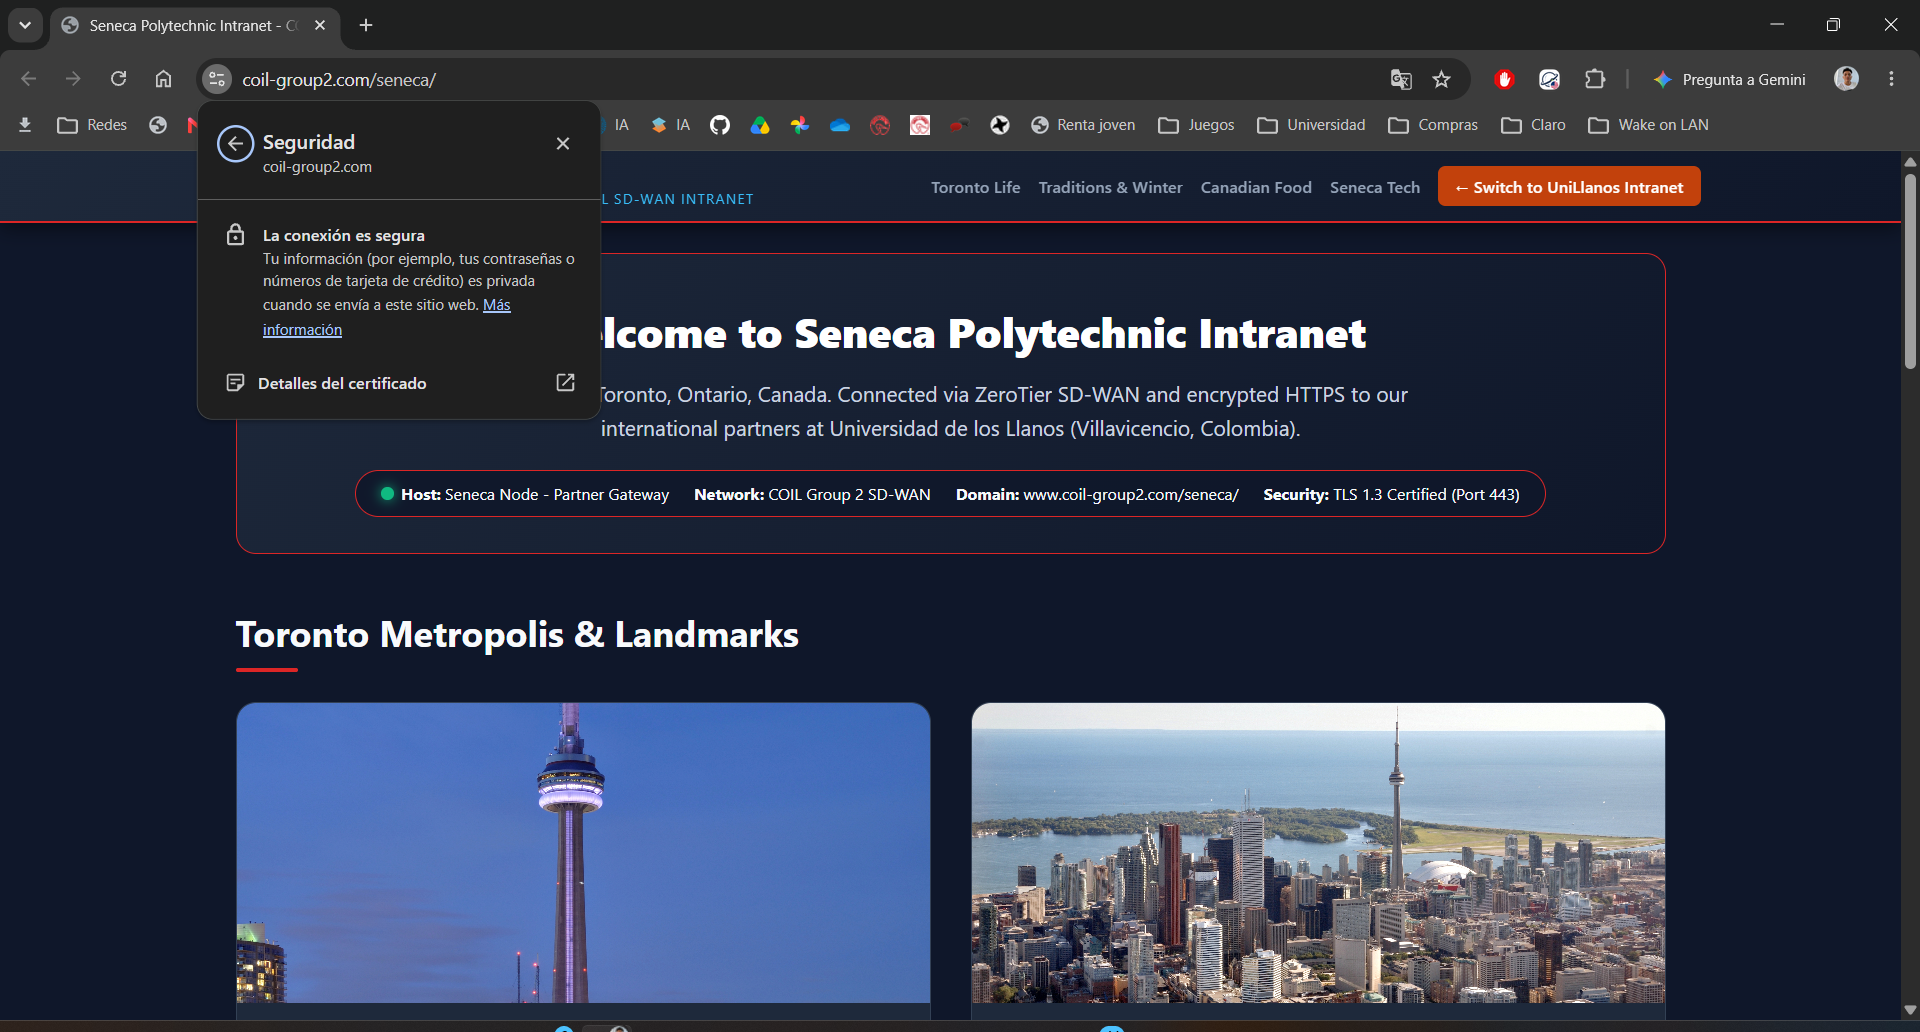
\includegraphics[width=0.90\textwidth]{figuras/cert_chrome_trusted_fresh.png}
\caption{Live Google Chrome verification on Windows navigating to \texttt{https://www.coil-group2.com/seneca/} with the site security panel open, demonstrating trusted HTTPS status and zero certificate warnings after Root CA installation (bonus objective).}
\label{fig:cert_chrome_trusted}
\end{figure*}

\begin{figure*}[htbp]
\centering
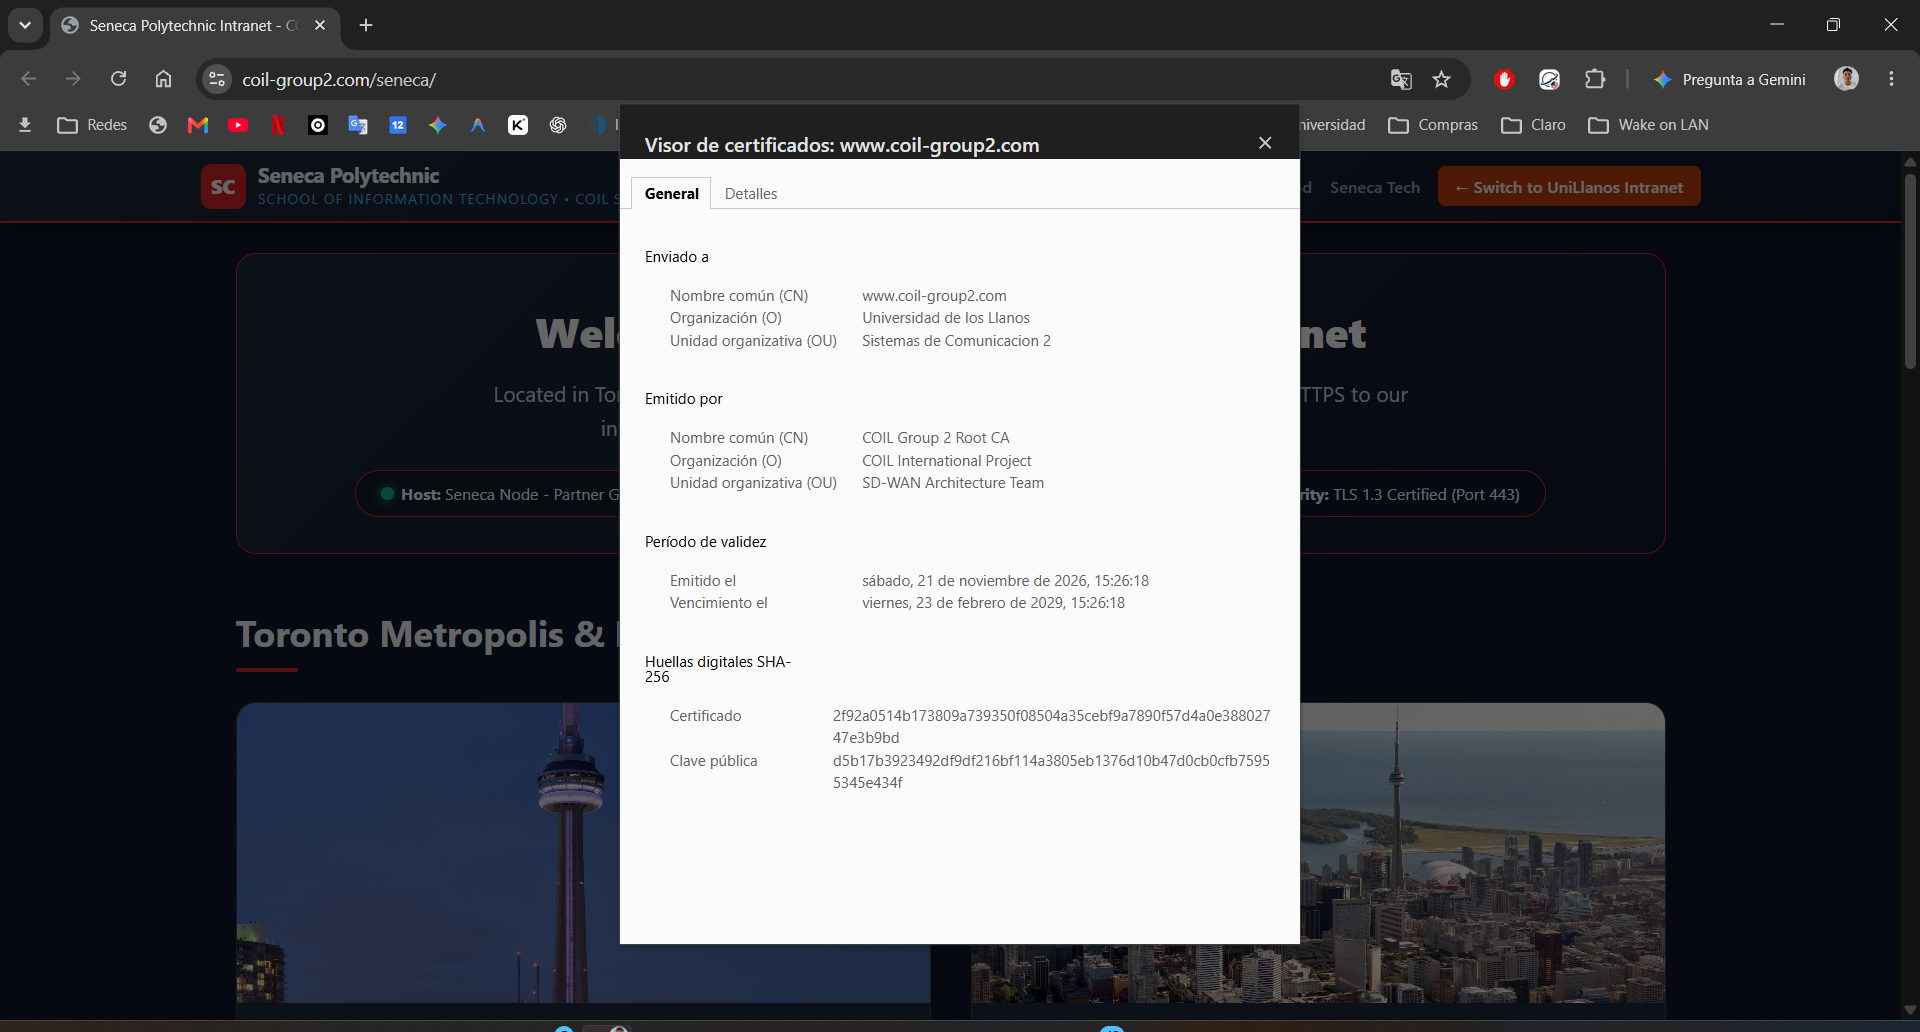
\includegraphics[width=0.90\textwidth]{figuras/cert_viewer_details_fresh.png}
\caption{Native X.509 Certificate Viewer inspection confirming the validated trust chain from \texttt{COIL Group 2 Root CA} to leaf certificate \texttt{www.coil-group2.com} with SHA-256 RSA-2048 signatures and SAN extensions.}
\label{fig:cert_viewer}
\end{figure*}

\begin{figure}[htbp]
\centering
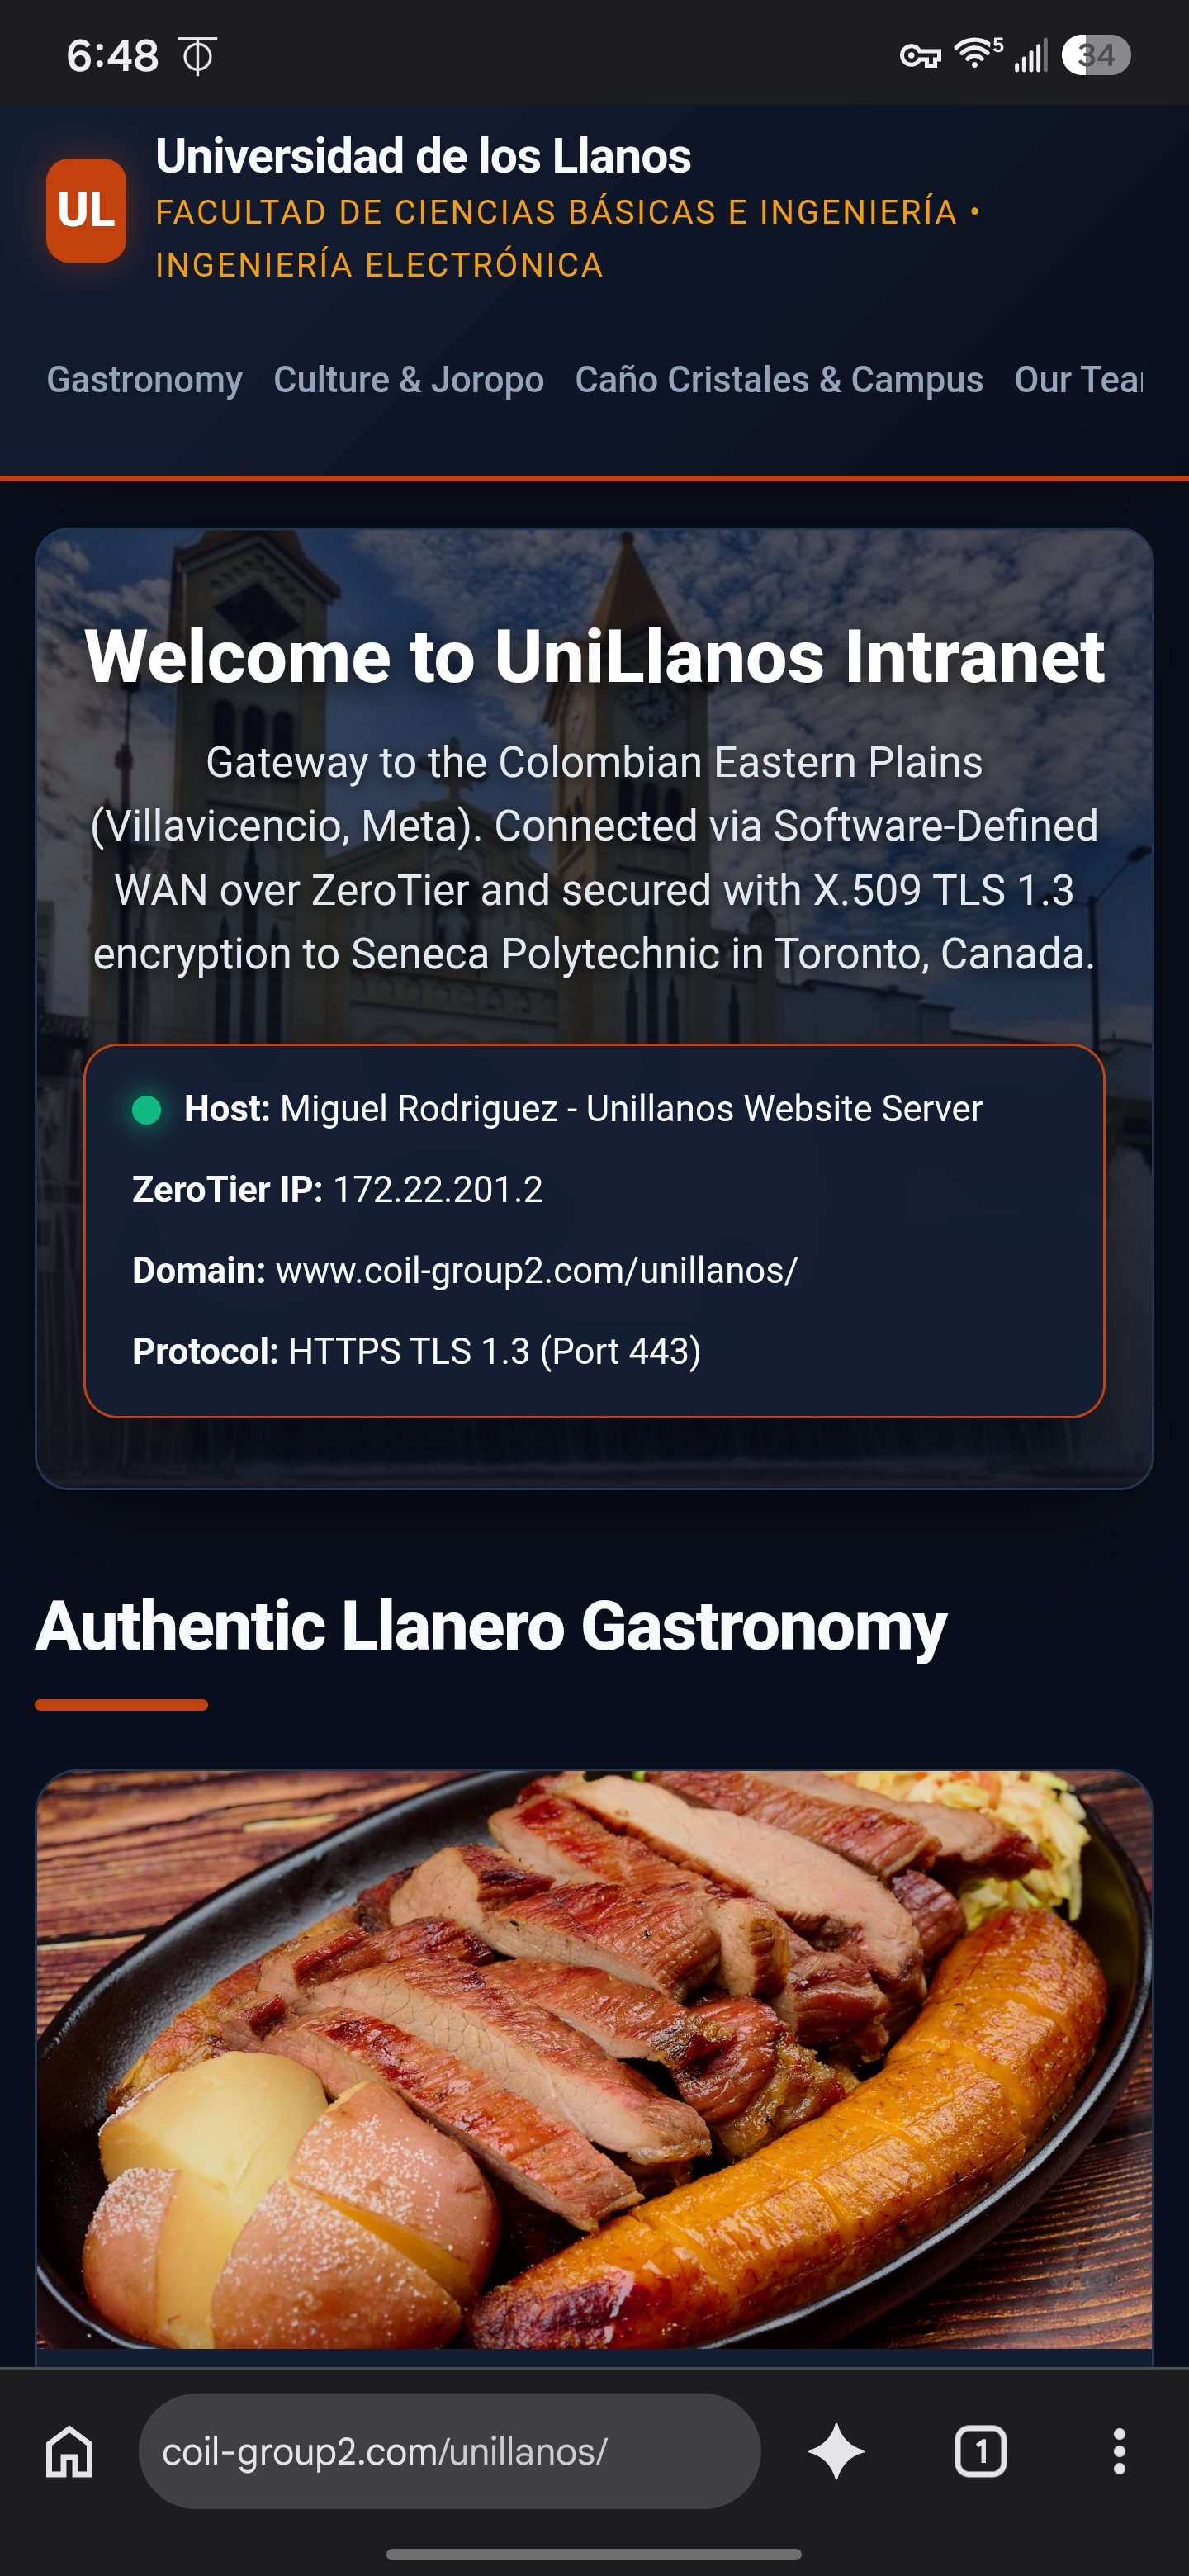
\includegraphics[width=0.58\columnwidth]{figuras/cert_mobile_android.jpg}
\caption{Cross-platform mobile verification on Android (Samsung Galaxy S24+, ZeroTier VPN active in status bar) accessing \texttt{www.coil-group2.com/unillanos/} over TLS~1.3 with the Root CA installed.}
\label{fig:cert_mobile}
\end{figure}

\subsection{Manual 4 (15\%): Authoritative and Forwarding DNS Server Configuration}
\label{subsec:manual4_dns}

To enable seamless domain-based navigation (\texttt{www.coil-group2.com/unillanos/} and \texttt{www.coil-group2.com/seneca/}) across all SD-WAN nodes without relying solely on manual IP entry, a dedicated Python DNS daemon (\texttt{modulo2/dns/dns\_server.py}) was implemented using the \texttt{dnslib} packet engine in compliance with RFC~1034~\cite{rfc1034}, RFC~1035~\cite{rfc1035}, and RFC~2308~\cite{rfc2308}. Figure~\ref{fig:dns_flowchart} illustrates the server's four-way packet-processing pipeline and host integration parameters.

\begin{figure*}[htbp]
\centering
% Local semantic palette (self-contained for drop-in inclusion in any preamble)
\definecolor{dnsNavy}{HTML}{1B365D}
\definecolor{dnsNavyBg}{HTML}{EEF4FB}
\definecolor{dnsBlue}{HTML}{1D4ED8}
\definecolor{dnsBlueBg}{HTML}{EFF6FF}
\definecolor{dnsTeal}{HTML}{0F766E}
\definecolor{dnsTealBg}{HTML}{F0FDFA}
\definecolor{dnsAmber}{HTML}{B45309}
\definecolor{dnsAmberBg}{HTML}{FFFBEB}
\definecolor{dnsRed}{HTML}{B91C1C}
\definecolor{dnsRedBg}{HTML}{FEF2F2}
\definecolor{dnsSlate}{HTML}{334155}
\definecolor{dnsMuted}{HTML}{64748B}
\definecolor{dnsPanelBg}{HTML}{F8FAFC}
\definecolor{dnsBorder}{HTML}{CBD5E1}

\resizebox{0.96\textwidth}{!}{%
\begin{tikzpicture}[
    >=Stealth,
    font=\scriptsize,
    node distance=0.55cm and 0.72cm,
    % Base box styles
    procbox/.style={
        rectangle,
        rounded corners=4pt,
        draw=dnsNavy,
        fill=dnsNavyBg,
        line width=0.85pt,
        text width=3.48cm,
        align=center,
        inner xsep=5pt,
        inner ysep=5pt,
        text=dnsSlate
    },
    parsebox/.style={
        procbox,
        draw=dnsSlate,
        fill=dnsPanelBg
    },
    decision/.style={
        diamond,
        aspect=2.2,
        draw=dnsBlue,
        fill=dnsBlueBg,
        line width=0.9pt,
        text width=2.45cm,
        align=center,
        inner xsep=3pt,
        inner ysep=3pt,
        text=dnsNavy
    },
    outcard/.style={
        rectangle,
        rounded corners=4pt,
        line width=0.9pt,
        text width=5.15cm,
        align=left,
        inner xsep=6pt,
        inner ysep=5pt,
        text=dnsSlate
    },
    outteal/.style={outcard, draw=dnsTeal, fill=dnsTealBg},
    outamber/.style={outcard, draw=dnsAmber, fill=dnsAmberBg},
    outred/.style={outcard, draw=dnsRed, fill=dnsRedBg},
    fwdbox/.style={
        rectangle,
        rounded corners=4pt,
        draw=dnsBlue,
        fill=dnsBlueBg,
        line width=0.9pt,
        text width=2.85cm,
        align=left,
        inner xsep=6pt,
        inner ysep=5pt,
        text=dnsSlate
    },
    relaybox/.style={
        rectangle,
        rounded corners=4pt,
        draw=dnsBlue,
        fill=dnsPanelBg,
        line width=0.9pt,
        text width=1.65cm,
        align=center,
        inner xsep=5pt,
        inner ysep=5pt,
        text=dnsSlate
    },
    dropbox/.style={
        rectangle,
        rounded corners=3pt,
        draw=dnsRed,
        dashed,
        fill=dnsRedBg,
        line width=0.75pt,
        text width=2.95cm,
        align=center,
        inner xsep=4pt,
        inner ysep=4pt,
        text=dnsRed
    },
    egressbox/.style={
        rectangle,
        rounded corners=4pt,
        draw=dnsNavy,
        fill=dnsNavyBg,
        line width=0.95pt,
        text width=2.15cm,
        align=center,
        inner xsep=5pt,
        inner ysep=6pt,
        text=dnsNavy
    },
    % Connectors & badges
    flow/.style={->, >=Stealth, line width=0.85pt, color=dnsNavy},
    flowteal/.style={->, >=Stealth, line width=0.95pt, color=dnsTeal},
    flowamber/.style={->, >=Stealth, line width=0.9pt, color=dnsAmber},
    flowred/.style={->, >=Stealth, line width=0.9pt, color=dnsRed},
    flowblue/.style={->, >=Stealth, line width=0.9pt, color=dnsBlue},
    dropflow/.style={->, >=Stealth, dashed, line width=0.75pt, color=dnsRed},
    yesbadge/.style={
        rectangle,
        rounded corners=2pt,
        fill=white,
        draw=dnsTeal,
        line width=0.55pt,
        inner xsep=3pt,
        inner ysep=1.5pt,
        font=\tiny\bfseries,
        text=dnsTeal
    },
    nobadge/.style={
        rectangle,
        rounded corners=2pt,
        fill=white,
        draw=dnsSlate,
        line width=0.55pt,
        inner xsep=3pt,
        inner ysep=1.5pt,
        font=\tiny\bfseries,
        text=dnsSlate
    },
    yesredbadge/.style={
        yesbadge,
        draw=dnsRed,
        text=dnsRed
    },
    yesamberbadge/.style={
        nobadge,
        draw=dnsAmber,
        text=dnsAmber
    },
    nobluebadge/.style={
        nobadge,
        draw=dnsBlue,
        text=dnsBlue
    },
    zonebox/.style={
        rectangle,
        rounded corners=6pt,
        draw=dnsBorder,
        fill=white,
        line width=0.85pt
    },
    zonehdr/.style={
        font=\footnotesize\bfseries,
        text=dnsNavy,
        inner sep=1pt
    },
    paramcard/.style={
        rectangle,
        rounded corners=4pt,
        draw=dnsBorder,
        fill=dnsPanelBg,
        line width=0.8pt,
        align=left,
        inner xsep=6pt,
        inner ysep=5pt,
        text=dnsSlate
    }
]

% ==============================================================================
% 1. TOP ZONE: PACKET-HANDLING DECISION PIPELINE (Right-to-Left by Construction)
% ==============================================================================

% Column 4: Four Resolution Lanes
\node[outteal] (out_a) at (0,0) {
    {\color{dnsTeal}\textbf{Authoritative \texttt{A} Record}} \hfill {\tiny\texttt{AA=1, NOERROR}}\\[2pt]
    Answer: \texttt{172.22.201.2} $\cdot$ TTL = \qty{300}{\second}\\
    Measured SD-WAN RTT: \textbf{\qty{0.53}{\milli\second}}
};

\node[outamber, below=0.38cm of out_a] (out_nodata) {
    {\color{dnsAmber}\textbf{RFC 2308 \texttt{NODATA + SOA}}} \hfill {\tiny\texttt{NOERROR, 0 Ans}}\\[2pt]
    Non-\texttt{A}/\texttt{ANY} (\texttt{AAAA} [28], \texttt{HTTPS} [65])\\
    Prevents Android \texttt{netd} \texttt{FORMERR} via \texttt{SOA} (\qty{300}{\second})
};

\node[outred, below=0.52cm of out_nodata] (out_nx) {
    {\color{dnsRed}\textbf{Authoritative \texttt{NXDOMAIN + SOA}}} \hfill {\tiny\texttt{RCODE=3}}\\[2pt]
    Unknown \texttt{*.coil-group2.com} subdomain\\
    Auth \texttt{SOA} negative cache (\texttt{TTL = \qty{300}{\second}})
};

\node[fwdbox, below=0.38cm of out_nx.south west, anchor=north west] (fwd_udp) {
    {\color{dnsBlue}\textbf{Upstream Forwarder}}\\[2pt]
    Raw UDP $\rightarrow$ \texttt{8.8.8.8:53}\\
    Socket timeout: \qty{2.0}{\second}
};

\node[relaybox, anchor=east] (out_relay) at (out_a.east |- fwd_udp.east) {
    {\color{dnsBlue}\textbf{Relay Reply}}\\[2pt]
    Pass upstream\\response
};

\node[dropbox, below=0.38cm of fwd_udp, text width=2.85cm] (drop_timeout) {
    Timeout / Error: Silent Drop
};

% Column 3: Secondary Decisions (Centered on Lane Pairs)
\coordinate (mid_dec1a) at ($(out_a.west)!0.5!(out_nodata.west)$);
\node[decision, anchor=east] (dec1a) at ($(mid_dec1a)+(-1.00cm,0)$) {
    \texttt{qtype in}\\[1pt]\texttt{(A, ANY)}?
};

\coordinate (mid_dec2) at ($(out_nx.west)!0.5!(fwd_udp.west)$);
\node[decision, anchor=east] (dec2) at ($(mid_dec2)+(-1.00cm,0)$) {
    Subdomain of\\[1pt]\texttt{coil-group2.com}?
};

% Column 2: Primary Decision (Centered between Dec 1a and Dec 2)
\coordinate (mid_dec1) at ($(dec1a.west)!0.5!(dec2.west)$);
\node[decision, anchor=east] (dec1) at ($(mid_dec1)+(-1.00cm,0)$) {
    \texttt{qname in}\\[1pt]\texttt{DOMAINS}?
};

% Column 1: Ingress, Parsing & Error Drop
\node[parsebox, left=0.72cm of dec1.west] (parser) {
    {\color{dnsNavy}\textbf{Parse \& Normalize}}\\[2pt]
    \texttt{DNSRecord.parse(data)}\\
    Lowercase \texttt{qname} (strip `\texttt{.}'), \texttt{qtype}
};

\node[procbox, above=0.55cm of parser] (ingress) {
    {\color{dnsNavy}\textbf{UDP Ingress Socket}}\\[2pt]
    Bind \texttt{0.0.0.0:53} (\texttt{recvfrom(4096)})\\
    \texttt{SIO\_UDP\_CONNRESET=False}
};

\node[dropbox, below=0.55cm of parser] (drop_invalid) {
    Invalid Packet: Silent Drop
};

% Column 5: Unified Client Egress Collector
\coordinate (egress_rail_x) at ($(out_a.east)+(0.48cm,0)$);
\coordinate (egress_top) at (egress_rail_x |- out_a.east);
\coordinate (egress_mid) at ($(out_a.east)!0.5!(out_relay.east)$);
\coordinate (egress_bot) at (egress_rail_x |- out_relay.east);
\coordinate (egress_hub) at (egress_rail_x |- egress_mid);

\node[egressbox, right=0.42cm of egress_hub] (egress) {
    \textbf{Client Reply}\\[2pt]
    \texttt{sendto(pkt, addr)}\\
    SD-WAN Peer
};

% ==============================================================================
% 2. ORTHOGONAL CONNECTORS & EDGE BADGES (Zero Absolute Coords, Zero Piercing)
% ==============================================================================

% Ingress -> Parser -> Dec1
\draw[flow] (ingress.south) -- (parser.north);
\draw[flow] (parser.east) -- (dec1.west);
\draw[dropflow] (parser.south) -- node[right, font=\tiny, text=dnsRed, xshift=2pt] {Parse Error} (drop_invalid.north);

% Dec1 -> Dec1a / Dec2
\draw[flowteal] (dec1.north) |- (dec1a.west);
\coordinate (b_dec1_yes) at ($(dec1.east |- dec1a.west)!0.5!(dec1a.west)$);
\node[yesbadge] at (b_dec1_yes) {YES};

\draw[flowblue] (dec1.south) |- (dec2.west);
\coordinate (b_dec1_no) at ($(dec1.east |- dec2.west)!0.5!(dec2.west)$);
\node[nobadge] at (b_dec1_no) {NO};

% Dec1a -> Out A / Out NODATA
\draw[flowteal] (dec1a.north) |- (out_a.west);
\coordinate (b_dec1a_yes) at ($(dec1a.east |- out_a.west)!0.5!(out_a.west)$);
\node[yesbadge] at (b_dec1a_yes) {YES};

\draw[flowamber] (dec1a.south) |- (out_nodata.west);
\coordinate (b_dec1a_no) at ($(dec1a.east |- out_nodata.west)!0.5!(out_nodata.west)$);
\node[yesamberbadge] at (b_dec1a_no) {NO};

% Dec2 -> Out NXDOMAIN / Forwarder
\draw[flowred] (dec2.north) |- (out_nx.west);
\coordinate (b_dec2_yes) at ($(dec2.east |- out_nx.west)!0.5!(out_nx.west)$);
\node[yesredbadge] at (b_dec2_yes) {YES};

\draw[flowblue] (dec2.south) |- (fwd_udp.west);
\coordinate (b_dec2_no) at ($(dec2.east |- fwd_udp.west)!0.5!(fwd_udp.west)$);
\node[nobluebadge] at (b_dec2_no) {NO};

% Forwarder -> Relay & Timeout Drop
\draw[flowblue] (fwd_udp.east) -- (out_relay.west);
\draw[dropflow] (fwd_udp.south) -- node[right, font=\tiny, text=dnsRed, xshift=2pt] {\texttt{resp=None}} (drop_timeout.north);

% Egress Collector Rail -> Client Reply
\draw[line width=0.85pt, color=dnsNavy] (egress_top) -- (egress_bot);
\draw[line width=0.85pt, color=dnsTeal] (out_a.east) -- (egress_rail_x |- out_a.east);
\draw[line width=0.85pt, color=dnsAmber] (out_nodata.east) -- (egress_rail_x |- out_nodata.east);
\draw[line width=0.85pt, color=dnsRed] (out_nx.east) -- (egress_rail_x |- out_nx.east);
\draw[line width=0.85pt, color=dnsBlue] (out_relay.east) -- (egress_rail_x |- out_relay.east);
\foreach \pt in {egress_top, egress_bot, egress_hub} {
    \fill[dnsNavy] (\pt) circle (1.4pt);
}
\fill[dnsAmber] (egress_rail_x |- out_nodata.east) circle (1.4pt);
\fill[dnsRed] (egress_rail_x |- out_nx.east) circle (1.4pt);
\draw[flow] (egress_hub) -- (egress.west);

% Pipeline Bounding Box & Section A Header
\node[fit=(ingress)(parser)(drop_invalid)(dec1)(dec1a)(dec2)(out_a)(out_nodata)(out_nx)(fwd_udp)(drop_timeout)(out_relay)(egress), inner sep=0pt] (pipe_bbox) {};
\node[zonehdr, anchor=south west] (hdr_a) at ($(pipe_bbox.north west)+(0,0.22cm)$) {
    A. Authoritative \& Forwarding Packet-Handling Pipeline (\texttt{modulo2/dns/dns\_server.py} $\cdot$ \texttt{dnslib} Engine)
};

\begin{pgfonlayer}{bg}
\node[zonebox, fit=(pipe_bbox)(hdr_a), inner sep=8pt] (zone_a) {};
\end{pgfonlayer}

% ==============================================================================
% 3. BOTTOM ZONE: 3-COLUMN SYSTEM PARAMETERS & WINDOWS/ZEROTIER INTEGRATION
% ==============================================================================

\node[zonehdr, anchor=north west] (hdr_b) at ($(zone_a.south west)+(8pt,-0.40cm)$) {
    B. Zone Table, RFC 2308 SOA Authority Parameters \& Windows / ZeroTier Host Integration
};

% Compute equal widths for 3 flush parameter cards spanning zone_a width (minus inner padding)
\path let \p1 = (zone_a.west), \p2 = (zone_a.east),
          \n1 = {(\x2 - \x1 - 16pt - 0.70cm)/3 - 12pt} in
    node[paramcard, anchor=north west, text width=\n1, minimum height=2.35cm] (card_domains) at ($(hdr_b.south west)+(0,-0.16cm)$) {
        {\color{dnsTeal}\textbf{1. Authoritative \texttt{DOMAINS} Map}}\\[2pt]
        {\color{dnsBorder}\rule{\linewidth}{0.5pt}}\\[3pt]
        \begin{tabular*}{\linewidth}{@{}l@{\extracolsep{\fill}}r@{}}
        \texttt{www.coil-group2.com} & \texttt{172.22.201.2} \\
        \texttt{coil-group2.com} & \texttt{172.22.201.2} \\
        \texttt{unillanos.coil-group2.com} & \texttt{172.22.201.2} \\
        \texttt{seneca.coil-group2.com} & \texttt{172.22.201.2} \\
        \end{tabular*}\\[4pt]
        {\tiny\color{dnsMuted} Records: \texttt{QTYPE.A / ANY} $\cdot$ TTL: \qty{300}{\second} $\cdot$ \texttt{NOERROR}}
    }
    node[paramcard, anchor=north west, text width=\n1, minimum height=2.35cm] (card_soa) at ($(card_domains.north east)+(0.35cm,0)$) {
        {\color{dnsAmber}\textbf{2. \texttt{SOA} Authority (\texttt{coil-group2.com})}}\\[2pt]
        {\color{dnsBorder}\rule{\linewidth}{0.5pt}}\\[3pt]
        \begin{tabular*}{\linewidth}{@{}l@{\extracolsep{\fill}}r@{}}
        Primary NS (\texttt{MNAME}): & \texttt{ns.coil-group2.com} \\
        Admin (\texttt{RNAME}): & \texttt{admin.coil-group2.com} \\
        Serial / Min TTL: & \texttt{2026112101} / \qty{300}{\second} \\
        Ref / Ret / Exp: & \qty{3600}{\second} / \qty{600}{\second} / \qty{86400}{\second} \\
        \end{tabular*}\\[4pt]
        {\tiny\color{dnsMuted} Returned in \texttt{auth} section (\qty{300}{\second}) for \texttt{NODATA}/\texttt{NXDOMAIN}}
    }
    node[paramcard, anchor=north west, text width=\n1, minimum height=2.35cm] (card_host) at ($(card_soa.north east)+(0.35cm,0)$) {
        {\color{dnsNavy}\textbf{3. Windows \& ZeroTier SD-WAN Integration}}\\[2pt]
        {\color{dnsBorder}\rule{\linewidth}{0.5pt}}\\[3pt]
        \textbf{ICS Port Release:} Stop \texttt{SharedAccess} (frees UDP/53).\\[1.5pt]
        \textbf{Firewall Rule:} Allow inbound \texttt{COIL\_DNS\_53} (UDP/53).\\[1.5pt]
        \textbf{ZeroTier Push:} Net \texttt{abfd31bd47affa39} pushes domain \texttt{coil-group2.com} \& NS \texttt{172.22.201.2} (\texttt{hosts} fallback).
    };

\begin{pgfonlayer}{bg}
\node[zonebox, fit=(hdr_b)(card_domains)(card_soa)(card_host), inner sep=8pt] (zone_b) {};
\end{pgfonlayer}

\end{tikzpicture}%
}
\caption{Packet-handling decision pipeline and authoritative zone configuration of the \texttt{dnslib}-based DNS daemon (\texttt{modulo2/dns/}\allowbreak\texttt{dns\_server.py}). Incoming UDP/53 datagrams are parsed, normalized, and routed across four deterministic branches: authoritative \texttt{A} resolution (\texttt{172.22.201.2}, TTL~=~\qty{300}{\second}, measured SD-WAN RTT~=~\qty{0.53}{\milli\second}), RFC~2308 \texttt{NODATA+SOA} responses preventing Android \texttt{netd} \texttt{FORMERR} faults on \texttt{AAAA}/\texttt{HTTPS} queries, \texttt{NXDOMAIN+SOA} negative caching for unregistered subdomains, and raw UDP forwarding to \texttt{8.8.8.8:53} (\qty{2.0}{\second} timeout) for external domains.}
\label{fig:dns_flowchart}
\end{figure*}


\subsubsection{Step 1: Authoritative Zone and RFC 2308 Negative Caching Engine}
The DNS daemon binds \texttt{UDP 0.0.0.0:53} (disabling Windows UDP connection-reset exceptions via \texttt{SIO\_UDP\_CONNRESET = False}) and maintains an authoritative dictionary mapping all four project hostnames (\texttt{www.coil-group2.com}, \texttt{coil-group2.com}, \texttt{unillanos.coil-group2.com}, and \texttt{seneca.coil-group2.com}) to \texttt{172.22.201.2} with a \qty{300}{\second} TTL:
\begin{itemize}
    \item \textbf{Type \texttt{A} (1) and \texttt{ANY} (255) Queries:} Returns an authoritative \texttt{NOERROR} answer with \texttt{AA=1} and \texttt{rdata=A("172.22.201.2")}.
    \item \textbf{Type \texttt{AAAA} (28) and \texttt{HTTPS} (65) Queries (\texttt{NODATA+SOA}):} Modern Chromium and Android (\texttt{netd}) resolvers issue parallel \texttt{AAAA} and \texttt{HTTPS} queries alongside \texttt{A} lookups. Under RFC~2308~\cite{rfc2308}, returning an empty answer section without an Authority \texttt{SOA} record causes Android \texttt{netd} to abort with \texttt{FORMERR}. The server therefore appends \texttt{SOA("ns.coil-group2.com", "admin.coil-group2.com", (2026112101, 3600, 600, 86400, 300))} in the authority section.
    \item \textbf{Unregistered Subdomains (\texttt{NXDOMAIN+SOA}):} Queries matching \texttt{*.coil-group2.com} outside the authoritative dictionary receive \texttt{RCODE.NXDOMAIN} with the authoritative \texttt{SOA} record.
    \item \textbf{External Internet Queries:} Non-COIL domains are forwarded over UDP to Google Public DNS (\texttt{8.8.8.8:53}, \qty{2.0}{\second} timeout) and relayed transparently back to the client.
\end{itemize}

\subsubsection{Step 2: Windows Port 53 Binding, Firewall Rules, and Headless Persistence}
On Windows 11, the Internet Connection Sharing service (\texttt{SharedAccess}) can reserve UDP port 53. Free port 53, open inbound firewall rules (\texttt{COIL\_DNS\_53}), and register the headless Scheduled Task (\texttt{COIL\_DNS\_Daemon} under \texttt{S4U} logon):

\begin{lstlisting}[caption={Provisioning UDP port 53, firewall rules, and persistent S4U DNS daemon.},label={lst:manual4_service}]
Stop-Service SharedAccess -Force -ErrorAction SilentlyContinue
New-NetFirewallRule -DisplayName "COIL_DNS_53" -Direction Inbound `
  -Protocol UDP -LocalPort 53 -Action Allow
$action = New-ScheduledTaskAction -Execute "python.exe" `
  -Argument '-u "modulo2\dns\dns_server.py"'
$principal = New-ScheduledTaskPrincipal -UserId (whoami) `
  -LogonType S4U -RunLevel Highest
Register-ScheduledTask -TaskName "COIL_DNS_Daemon" -Action $action `
  -Principal $principal -Force
Start-ScheduledTask -TaskName "COIL_DNS_Daemon"
\end{lstlisting}

\subsubsection{Step 3: ZeroTier DNS Push and Client Verification}
In ZeroTier Central (Figure~\ref{fig:zerotier_settings}), configure \texttt{SERVERS: 172.22.201.2} under the DNS panel. On Android clients, enable \textit{Use Network DNS} inside the ZeroTier One app and set Android \textit{Private DNS} to \textit{Off} so DNS-over-TLS does not bypass the SD-WAN resolver; on Windows clients without ZeroTier DNS push enabled, execute \texttt{modulo2/dns/setup\_hosts.ps1} as a deterministic local fallback. Live verification from both \texttt{172.22.201.2} and remote gateway \texttt{172.22.31.69} confirmed authoritative \texttt{A} and \texttt{SOA} resolution:

\begin{lstlisting}[caption={Live authoritative DNS verification for Type A and Type AAAA queries.},label={lst:manual4_verify}]
PS C:\> Resolve-DnsName www.coil-group2.com -Server 172.22.201.2 -Type A
Name                 Type   TTL   Section    IPAddress
----                 ----   ---   -------    ---------
www.coil-group2.com  A      300   Answer     172.22.201.2

PS C:\> Resolve-DnsName www.coil-group2.com -Server 172.22.201.2 -Type AAAA
Name             Type  TTL  Section    PrimaryServer       NameAdministrator     SerialNumber
----             ----  ---  -------    -------------       -----------------     ------------
coil-group2.com  SOA   300  Authority  ns.coil-group2.com  admin.coil-group2.com 2026112101
\end{lstlisting}

Figure~\ref{fig:ws_dns} presents the live Wireshark dissection of Frames~1 and~2 captured on the ZeroTier virtual adapter (\texttt{dns} display filter), confirming transaction ID \texttt{0x9121}, authoritative flag \texttt{AA=1}, resolved address \texttt{172.22.201.2} (\texttt{TTL = 300 s}), and a round-trip resolution latency of \qty{0.5346}{\milli\second}.

\begin{figure*}[htbp]
\centering
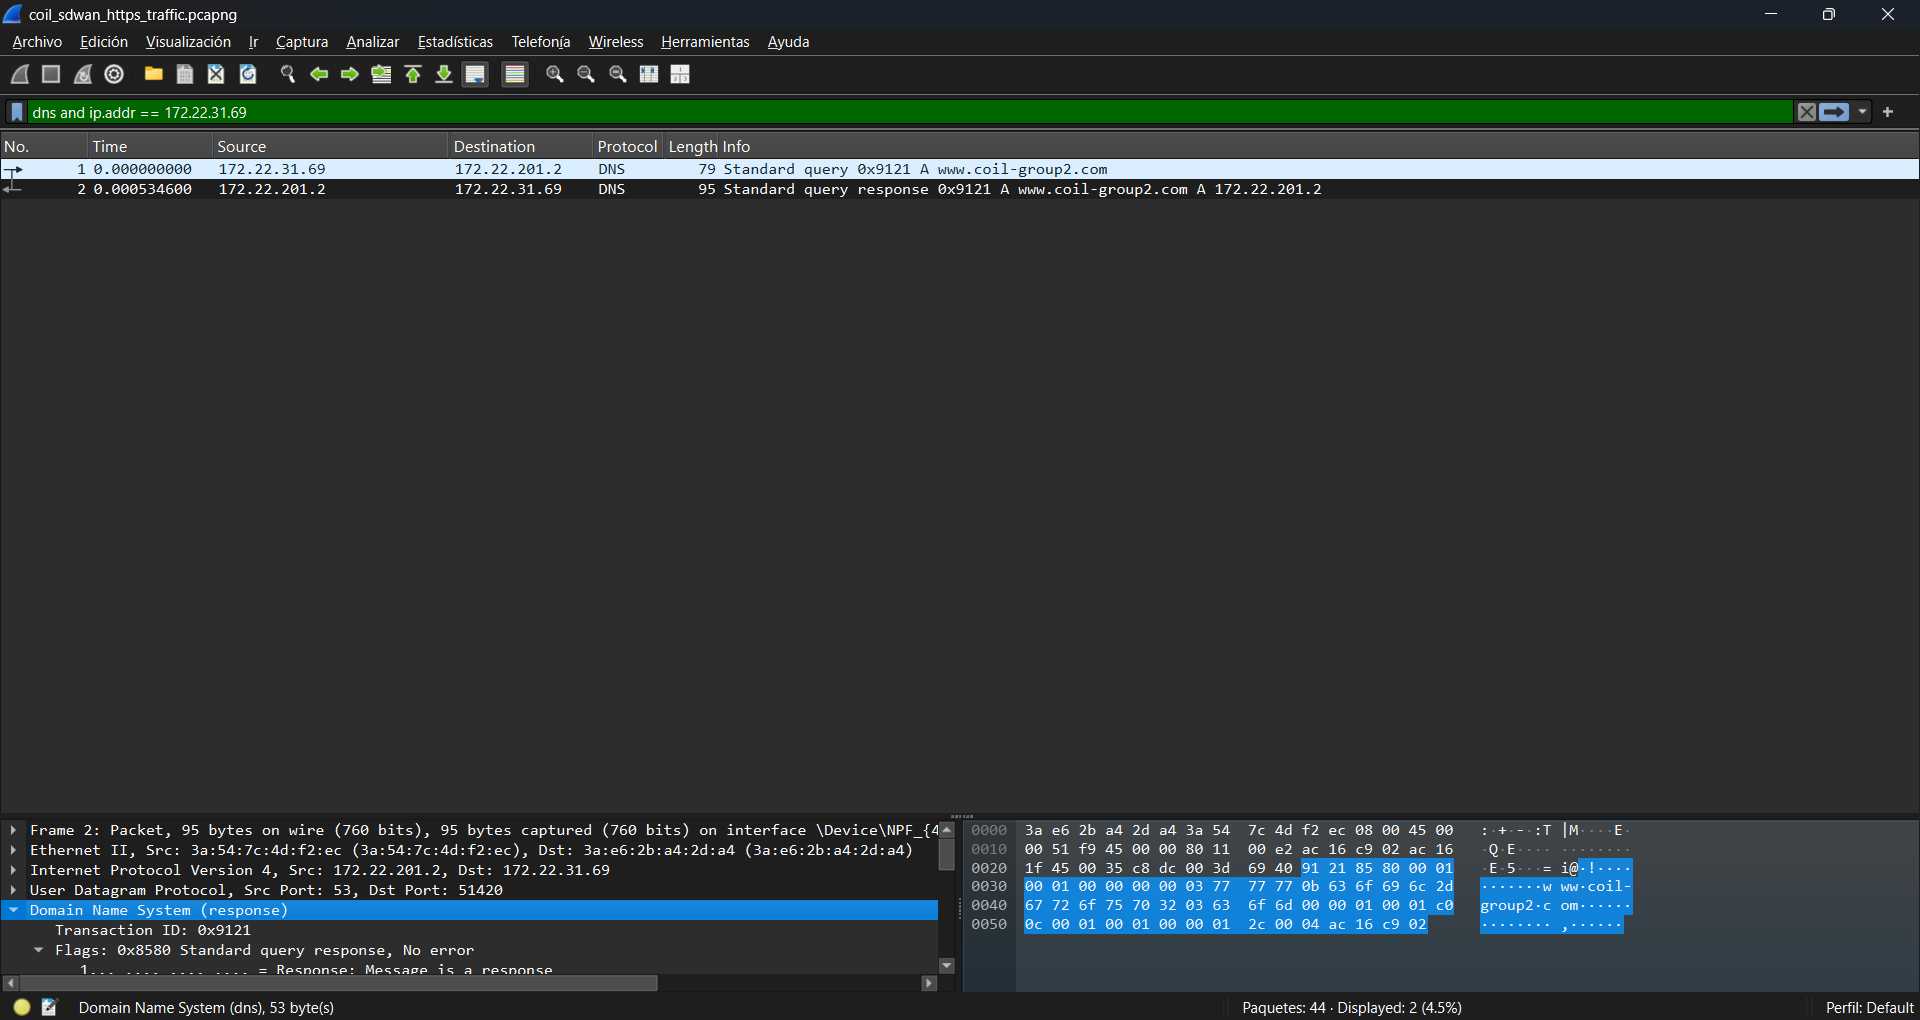
\includegraphics[width=0.92\textwidth]{figuras/wireshark_5_dns_resolution.png}
\caption{Wireshark protocol dissection of the live SD-WAN DNS query and authoritative response (Frames~1--2, Transaction ID \texttt{0x9121}, \qty{0.5346}{\milli\second} RTT) resolving \texttt{www.coil-group2.com} to \texttt{172.22.201.2} over UDP port 53.}
\label{fig:ws_dns}
\end{figure*}
